% ====================================================================
%+
% SECTION:
%    sn.tex  
%
% CHAPTER:
%    transients.tex  
%
% ELEVATOR PITCH:
%    Explain in a few sentences what the relevant discovery or
%    measurement is going to be discussed, and what will be important
%    about it. This is for the browsing reader to get a quick feel
%    for what this section is about.
%
% COMMENTS:
%
%
% BUGS:
%
%
% AUTHORS:
%   Federica Bianco (@fedhere)
%
% ====================================================================

\section{Supernovae as transients}
\def\secname{SNtransients}\label{sec:\secname} % For example, replace "keyword" with "lenstimedelays"

\credit{fedhere} % (Writing team)

Supernovae (SNe) represent the final dramatic stages of life of many
stars. The term SN we covers a diverse set of phenomena: explosion of
low mass stars in binary systems, thermonuclear SN or SN Ia (also
discussed in \ref{sec:supernovae}), and explosion of high mass stars,
Core collapse (CC) SNe, and even terminal explosions of more exotic
systems, yet to be understood, like Super Luminous SNe
(SLSNe). Phenomenologically, the observable of the explosion are
themselves diverse. The transient duration ranges between weeks and
months, years. The electromagnetic energy radiated ranges between
$\sim0.1$ (faintest CC SNe), to $\sim1$ (SN Ia) and $\sim100$ (SLSNe)
$\times 10^{49}$ erg, corresponding to absolute magnitudes at peak
ranging between $\sim-19$ and $\sim-22$.

LSST's contribution to SNe studies can can be substantial. Synoptic
surveys such as SDSS, SNLS, PTF, PanSTARRS have revolutionized our
understanding of SN over and over again, exposing their diversity,
and revealing different progenitor channels. LSST's first crucial
input will be discovery: the normal type Ia SN rate out to redshift
$z=1$ is estimated to be $\sim200 ~(\mathrm{sq. deg.})^{-1}$ per
year\footnote{\url{http://www.lsst.org/sites/default/files/docs/Wood-Vasey_086.11.pdf}},
and SN~Ia represent only about 1/4 of all SN
events~(Li10): tens of millions of stars will explode
within the LSST footprint every year. The key questions concerning
LSST SN science are:
\begin{itemize}
\item
LSST's SN discovery power, 
\item
LSST's discrimination power, 
\item
the quality of the statistical sample over time. 
\end{itemize}
The first and second topic are \emph{time sensitive}, while the latter
is not, although it is interesting to understand the pace at which a
science question can be advanced in the life time of LSST.

{\bf \emph{Discovery:}} the SN~Ia discovery is rate is a standard LSST time-domain metric: a
fraction of $\sim40\%$ SN~Ia are expected to be discovered pre-peak
luminosity within the standard LSST survey
(e.g. \opsimdbref{db:baseCadence}~Figure~\ref{fig:enigmaEarlySNe}). The
topic of SNe discovery is discussed in further detail in
\ref{sec:supernovae}.

The next step is then {\bf\emph{discrimination}}, and the question we need
to answer, for SNe as well as for most other transients, is: will LSST
photometry allow to distinguish SN from other transients, and to
distinguish the different types of SN? And further: will this be
achievable in time to appropriately direct follow-up efforts? This is
particularly difficult considering that photometric classification
schemes have only achieve modest performances in distinguishing, for
example SN~Ic from SN~Ia. As mentioned earlier in this chapter, the issue
of prompt classification is at the heart of the success of LSST
transient science, but it is too complex to tackle in this chapter,
while LSST's ability to assess whether a new transient is young is discussed
in Section~\ref{transientsAge}.

When a large statistical sample of SNe is generated, LSST's photometry
may allow to set constraints on the diversity of the sample, even as a
standalone survey, without the aid of follow-up efforts.
{\bf Thus LSST \emph{alone} can shed light on the diversity within the population of SN},
which in turn may constrain the genesis of the explosion.\footnote{Reliable typing of a SN and redshift determination may still require auxiliary data.} Outstanding
questions that can be answered by an LSST photometric sample include,
for example, what is the percentage of SN Ia that arise from a
\emph{double degenerate} (DD) progenitor system (a CO WD-WD binary), from a
\emph {single degenerate} (SD) system (a WD-MS or WD-RG binary), or a
\emph{merger} (a WD-WD binary with a He and a CO WD)
(citation). Answering this question may reduce the scatter in the
Hubble diagram, if SNe from different progenitors are shown to require
different standardization (citation). On the CC~SN side: the diversity
of SN sub-classes, and the relationship between them (is there a
phenomenological continuum or actually distinct classes, e.g. between
IIp-IIL, IIb-Ib?) is yet to be understood. Individual well studied
objects may answer these questions: individual SN Ia with tight
constraints on the progenitor system show that both single and double
degenerate progenitors exist (e.g. SN 2011fe, \citealt{Li11}, ~\citealt{Olling15} and
PTF 11kx, \citealt{Dilday12}). However, a statistical sample is needed
to set constraints on populations.

Thus the technical question to be answered is: how much detail can be
sacrificed in favor of sample size without compromising diagnostic
power? And the diagnostic power relies on color and sampling: thus
what is the trade-off between cadence in the same filter, and
observations in different filters. Specifically, transients can be
distinguished early from two photometric characteristics: rise time
and color. There is a tension between these observables, as discussed
in Section~\ref{transientsAge}. Obtaining colors relies of course on
obtaining photometry in different bands at within short time scales,
as close as possible to \emph{simultaneously}. However, assessing the
rise slope is best done with a single filter, so prompt
characterization also needs multiple epochs within a night, although
separated by at least a few hours, in the same filter. That is:
observing with different filters it is impossible (or very hard) to
separate shape from color. Colors of course allow to learn a lot more
about the statistical sample: as long as the epoch of peak is reliably
assessed coadded light curves can be studied \citep{Bianco11}.

\subsection{Distinguishing progenitor scenarios}
In this chapter, we envision and design a SN related metric that works
on a large sample (months, to years of LSST data) and assess the
ability to characterize the contribution of SN with specific features
to the global population: as a test case we will use the presence of
an early blue excess for SN type Ia, signature of interaction with a
companion, and thus of a SD progenitor. Equivalently, the presence of
an early blue excess in CC~SN could be assessed, signature of shock
breakout for CC SNe. The \emph{figure of merit} for this science case
is the time within the survey required to achieve a sufficiently large
sample of SNe satisfying proper quality criteria to enable to
distinguish populations with different contribution from DD and SD
progenitors.  To do this we rely on simulations of the observables of
the population for different sample sizes, on the
\texttt{transientAsciiMetric} to determine the detectability of
interacting, and non-interacting SNe, and on the
\texttt{colorGapMetric} to assess the gap between of detections in 2
filters.

We simulate interacting SNe from the Nugent templates \citep{Nugent02}
injecting the angle dependent effects of interaction with a companion
as simulated by \citep{Kasen10}, for a $2~M_\odot$ and a $6~M_\odot$
MS companion stars, and a $1~M_\odot$ RG companion, following the
procedure of ~\citep{Bianco11}. We create synthetic progenitor
population with a fraction of single degenerate progenitor systems
$0.05 < f_\mathrm{SD} < 0.6 $ in 0.05 intervals. For each population
we calculate colors at random epochs, with a granularity of 1 day
within the first 10 days after explosion by subtracting magnitudes at
the same epoch, or at epochs separated by 1 day, and we include the
effects of observational noise by generating datapoints from a draw
within Gaussian distribution centered at the color measured in the
previous step and with standard deviation $\sigma_\mathrm{pop} = 0.5$,
1, and 2. One such lightcurve, with maximal interaction effects, is shown in Figure \ref{fig:kasenlc}.
We generate populations of $N_\mathrm{pop}=100$,
~1000,~10000 observations for $g'-r'$, $u'-r'$, $g'-i'$, and
$u'-i'$. Because the effect is heavily chromatic and it dissipates
becoming essentially negligible by $r$ band, $u'-i'$ gives the most
leverage. However $g'$ and $r'$ are the best observed LSST bands in
most cadences, and these considerations drive our choice of colors to
be simulated. We perform Kolmogorov-Smirnoff ($KS$) an
Anderson-Darling ($AD$) tests to evaluate, as a function of the sample
size $N_\mathrm{pop}$, the ability to distinguish the different
contributions.

\begin{figure}[hbt]
\centerline{
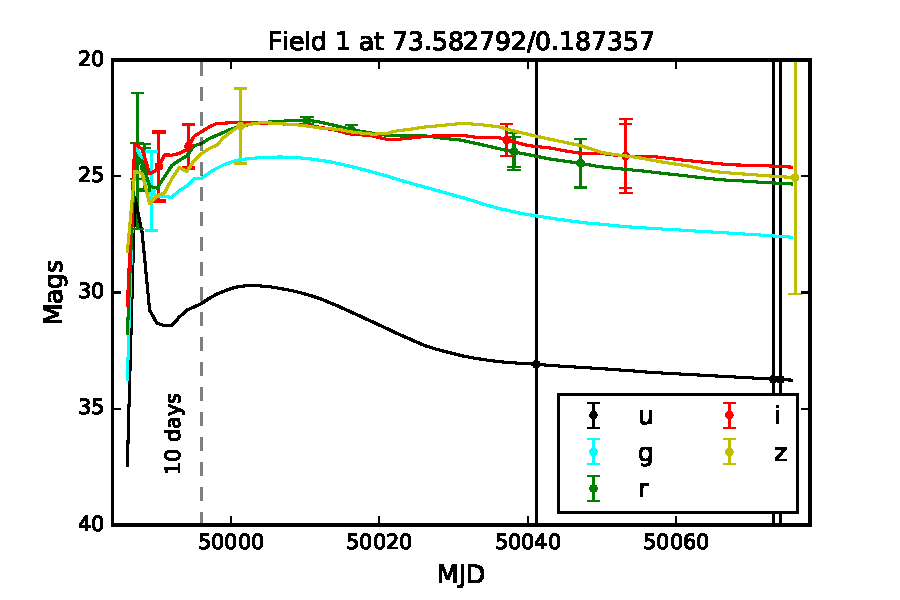
\includegraphics[width=0.6\textwidth]{figs/transients/LSST_Kasen_lcv0.pdf}
}
\caption{
A normal SN Ia lightcure at z=0.5 showing the effects of interaction with a RG companion as seen from the most favorable viewing angle: the effect is of interaction as simulated by \citet{Kasen10} is added on top of a lightcurve simulated from the \citealt{Nugent02} templates. The data points represent one possible LSST observations of this transient, obtained by running the \texttt{transientAsciiMetric}. This particular event is \emph{not} detected in two filters within the first 10 days after explosion, and it is thus a non-detection for our purpose.}
\label{fig:kasenlc}
\end{figure}



In the table below we report our diagnostic power, as the ability to distinguish a population with a $f_\mathrm{SD} > x$ from $f_\mathrm{SD}<0.05$ as a function of noise ($\sigma_\mathrm{pop}$) and population size ($N$)

\begin{center}
\begin{tabular}{ c | c| c| c | c | c| c| c | } 
$g-i$&\bf{$N$=100}&\bf{$N$=1,000}&\bf{$N$=10,000}& $g-r$&\bf{$N$=100}&\bf{$N$=1,000}&\bf{$N$=10,000} \\
  \hline
 \bf{$\sigma_\mathrm{pop} = 2.0$}&  -  & -  &  0.2 & &  -  & -  &  0.2 \\
 \bf{$\sigma_\mathrm{pop} = 1.0$}&  -  & 0.2 & 0.1 & &  -  & 0.2 & 0.1 \\
 \bf{$\sigma_\mathrm{pop} = 0.5$}& 0.4 & 0.1 & 0.1 & & 0.4 & 0.1 & 0.1 \\
&&&&&&&\\ $u-i$&\bf{$N$=100}&\bf{$N$=1,000}&\bf{$N$=10,000} & $u-r$&\bf{$N$=100}&\bf{$N$=1,000}&\bf{$N$=10,000}\\
 \bf{$\sigma_\mathrm{pop} = 2.0$}&  -  & -  &  0.2 & &  -  & -  &  0.2 \\
 \bf{$\sigma_\mathrm{pop} = 1.0$}&  -  & 0.2 & 0.1 & &  -  & 0.2 & 0.1 \\
 \bf{$\sigma_\mathrm{pop} = 0.5$}& 0.4 & 0.1 & 0.1 & & 0.4 & 0.1 & 0.1 \\

 \hline
\end{tabular}
\end{center}

At this point what remains to do is to evaluate how long it will take for a given LSST cadence to obtain a sufficient number of observations in the 2 desired colors, separated by less than 1 day, passing the SNR requirements. This should be done in a full Monte Carlo simulation injecting lightcurves with the proper lightcurve shape at the proper rate. However at this stage we simply evaluate the relative observability of SNe with excess, and SNe without excess, at $z~=~0.5$ and properly adjust the number of detections, according to the injected ratio. The relative detectability can be assessed with the \texttt{transientAsciiMetric}, injecting observations with realistic shapes, and we conclude that for RG progenitor the detectability is enhanced by $\sim50\%$.

Then we extract from the  \texttt{transientAsciiMetric}, injecting SN at $z=0.5$, the number of \emph{color observations} (observations in 2 bands within 1 day of each other, each fulfilling our SNR requirement for the color (which for simplicity we translate into a requirement on each observation of $\mathrm{SNR} > \frac{1.0}{2.0~\sigma_\mathrm{pop}/\sqrt{2}}$, which for $\sigma_\mathrm{pop}=2$ is $\mathrm{SNR}>1.5$) for 3-, 6-, and 12 months of survey in year 1.

With the minimum goal of distinguishing a SD contribution of 20\% to the SN Ia population, we need more than 1000 detections, in 2 filters within 1 day, with both datapoints in $SNR \geq 2$. With the  \texttt{transientAsciiMetric} we find that in $g'-r'$ color the baseline survey detects $\sim600$ such SNe in 3 months, $\sim1800$ in 6 months, $\sim9000$ in a year. But these pairs of observations are with any gap in time, within the first 10 days. To include the constraint that the detections should be within 24 hours we refer to the median inter-night gap metric, which is plotted in ~\ref{fig:enigmaGapAll} for the baseline survey, we estimate $~\sim10\%$ of the observation are revisited within a night. With the assumption that this is likely to happen in two different filters, which is \emph{non-conservative}, but neglecting intra-night observations that may happen in the two different filters, which is a \emph{conservative} assumption. Then our numbers drop by a factor 10 to $\sim60$ SNe in 3 months, $\sim180$ in 6 months, $\sim900$. Thus a year is \emph{nearly} enough for us to push our understanding of the progenitor population and constrain the fraction of SD progenitors to fractions smaller than 20\%. In the Table~\ref{tab:SummarySNprojs} we summarize the results of our metric for different LSST cadences, recalling that our figure of metric is the timeline in the LSST survey that enables us to distinguish a SD contribution of less than 20\%.

Figure~\ref{fig:sndetect} shows the detection rate for SN~Ia at $z=0.5$ in absence of shock interaction as a function of SNR (product of $g'$ and $r'$ limit) for 3, 6 months, and a year of \opsimdbref{db:baseCadence} (ideally I will plot it for the other survey as well tonight) 



\begin{table}
  \begin{tabular}{l|p{6cm}|c|c|c|c|p{5cm}}
    FoM & Brief description & {\rotatebox{90}{\opsimdbref{db:baseCadence}}}
	  & {\rotatebox{90}{\opsimdbref{db:NEOswithVisitTriplets}}} &
	  {\rotatebox{90}{\opsimdbref{db:NoVisitPairs}}} &
	  {\rotatebox{90}{\opsimdbref{db:opstwoPS}}} & Notes \\
    \hline
    \thesection-1 & \footnotesize{\texttt{SNIaprojenitorMetric},
    \texttt{1,000 detections}}      & ? & 1 & ? & ? &
    \footnotesize{Time to collect 10,00 relevant color observations in  years in 3 month intervals.} \\
    \thesection-2     & \footnotesize{\texttt{SNIaprojenitorMetric},
    \texttt{10,000 detections}}      & ? & ? & ? &? &
    \footnotesize{Time to collect 10,000 relevant color observations in  years in 3 month intervals.}\\
\end{tabular}
\caption{Figures-of-merit (FoMs) for statistical SN Ia progenitor studies to assess the contribution of SD progenitors to the SN Ia population.
}
\label{tab:SummarySNprojs}
\end{table}

\begin{figure}[hbt]
  \centerline{
    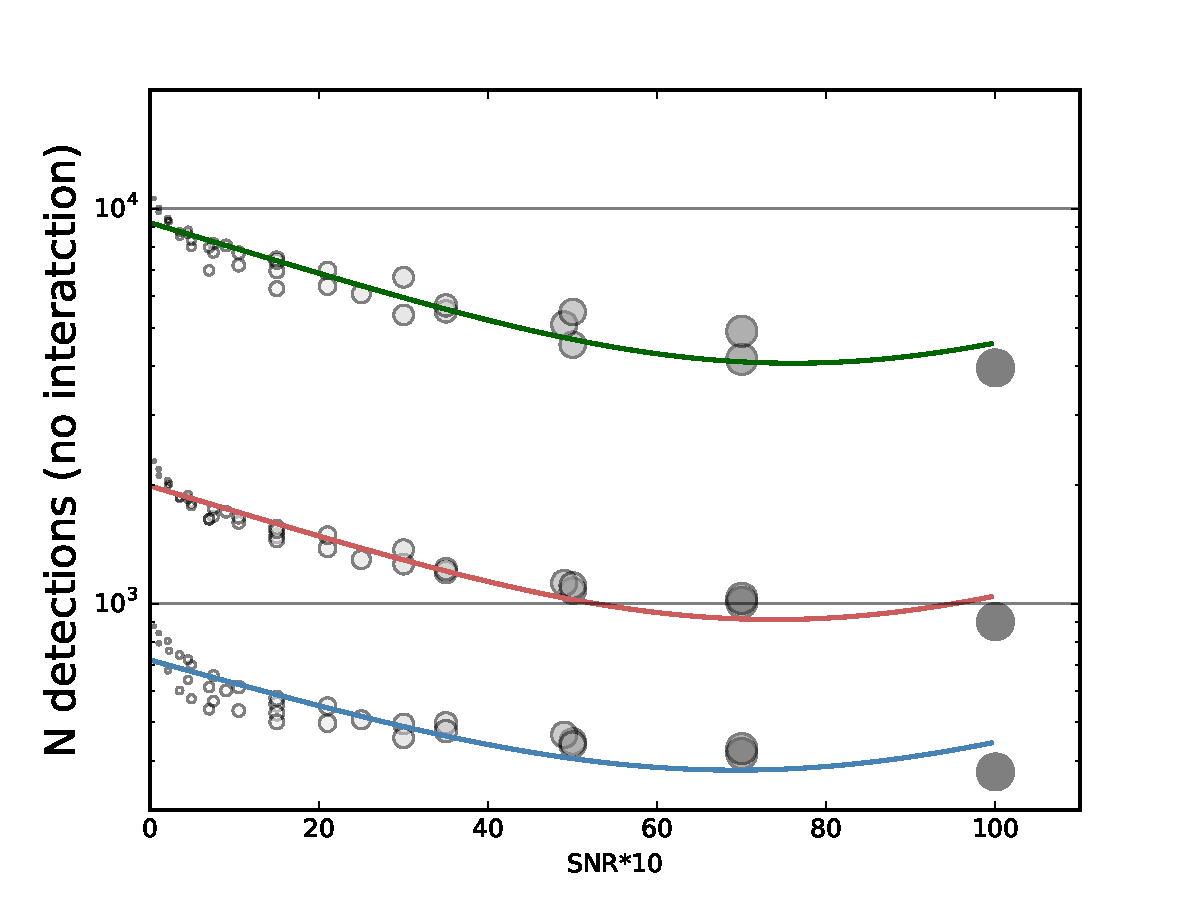
\includegraphics[width=0.6\textwidth]{figs/transients/LSST_Iadetected_wcolor.pdf}
  }
  \caption{
    Normal SN Ia lightcure at z=0.5 detected by the \opsimdbref{db:baseCadence} cadence in 3 months, 6 months, and 1 year, that provide color information useful to constrain the progenitor distribution. }
  \label{fig:sndetect}
\end{figure}

